\documentclass[a4paper]{article}

\usepackage{graphicx}
\graphicspath{{./figures/}}


\usepackage{url}  
 
\title{Higgs Triple Model Proposal}
\author{Ricardo Sanz, Víctor Gutiérrez}


\begin{document}

\maketitle

\section{Purpose}

The objective of the project is the development of a \textbf{simulation model of
a mobile robot} for use in different simulators: Gazebo \cite{Gazebo}, Webots\cite{Webots} and CoppeliaSim\cite{CoppeliaSim} simulators.

The final purpose if the models is to provide a virtual experimentation platform
to facilitate the development of autonomous controllers for UGVs. These models shall 
be used by future researchers in the development of control mechanisms for the robot.

\begin{figure}
\begin{center}
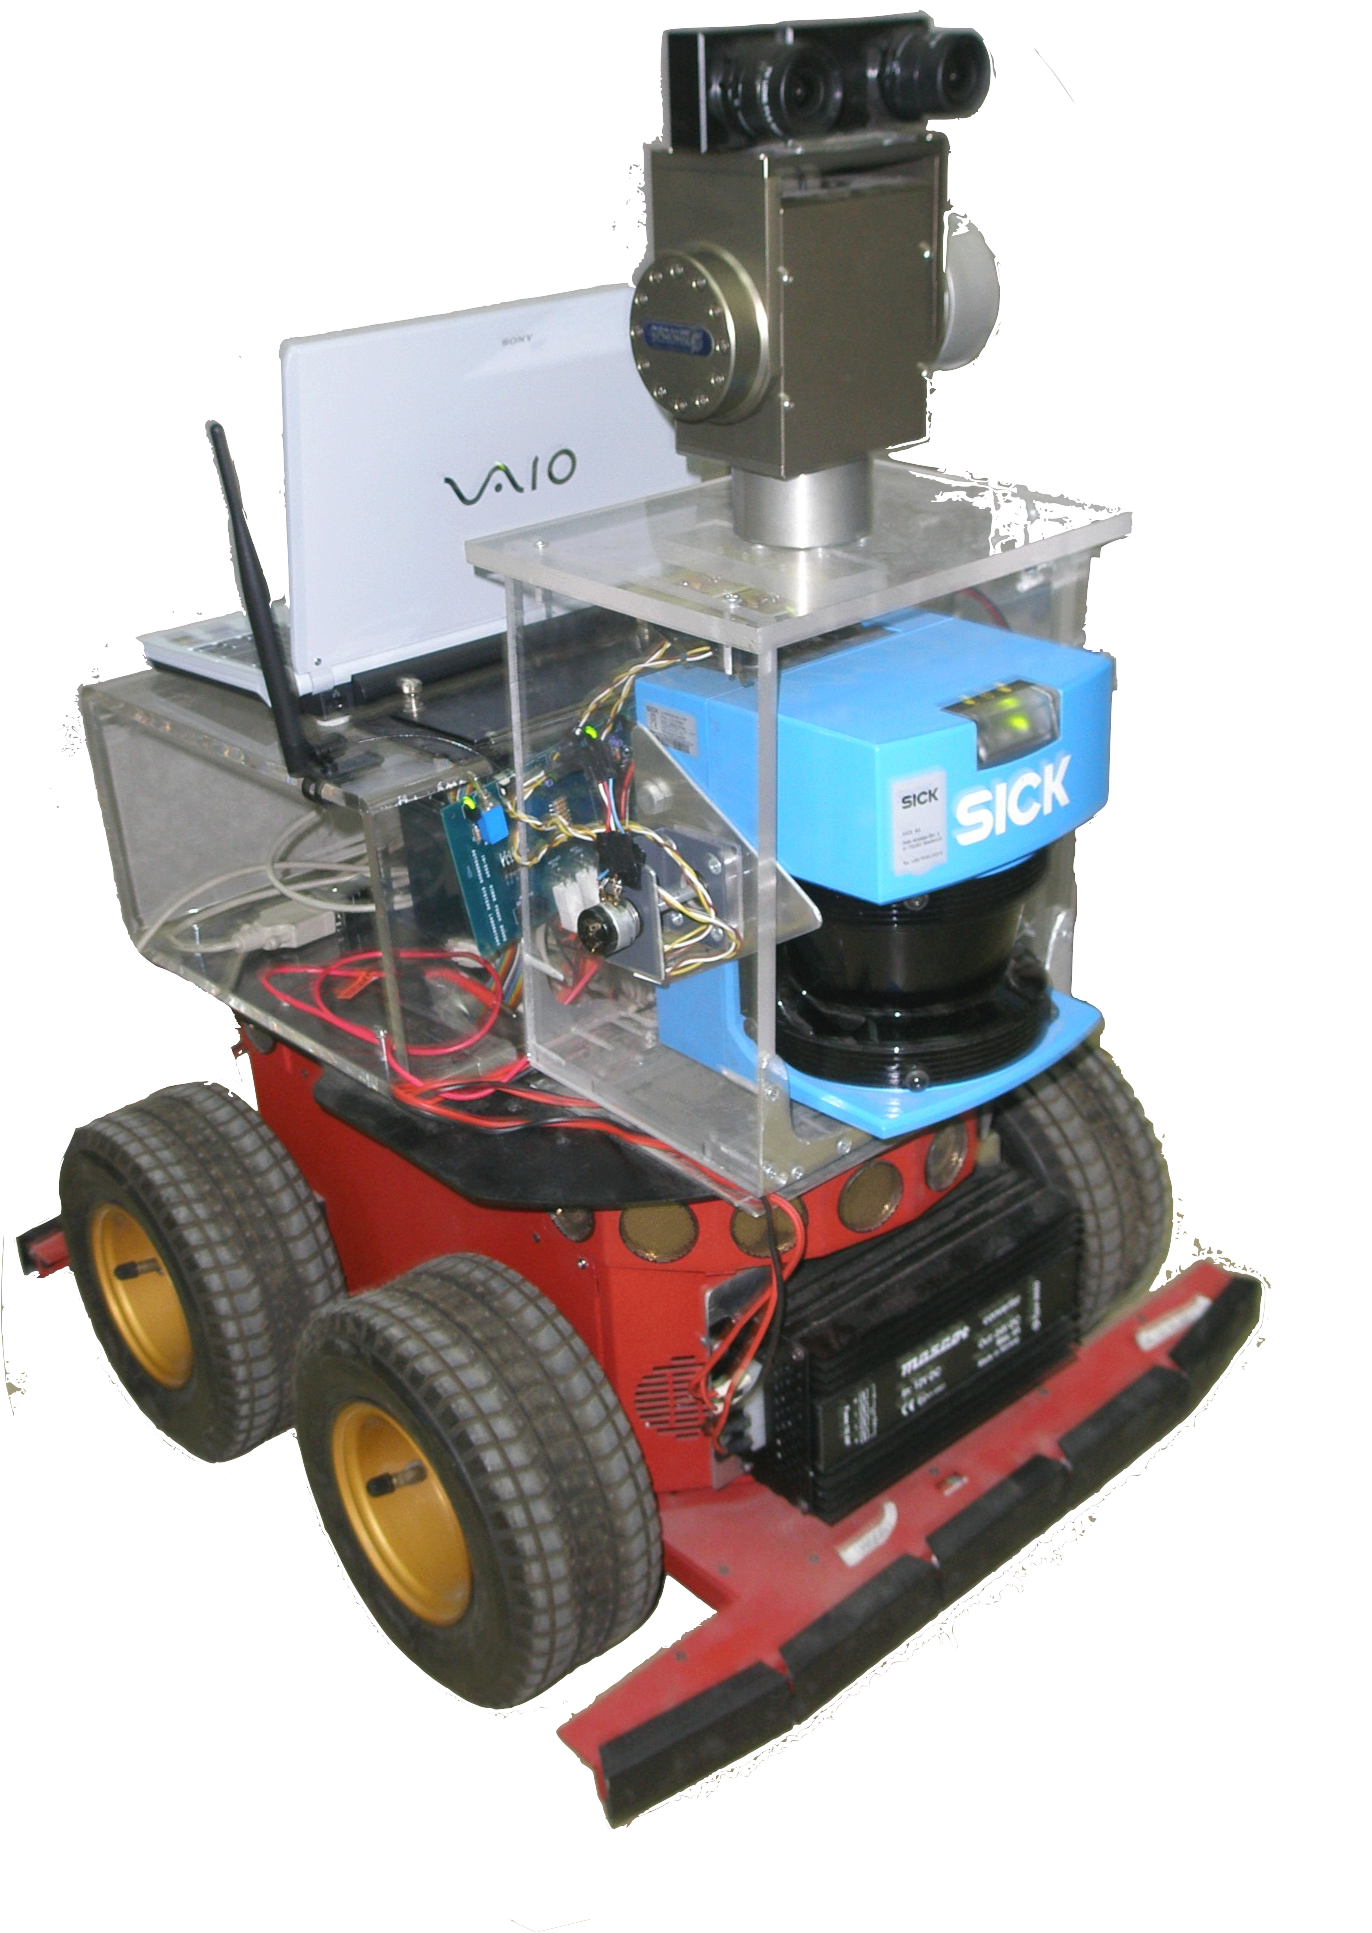
\includegraphics[width=7cm]{Higgs.png}
\caption{The Higgs robot.}
\label{fig:higgs}
\end{center}
\end{figure}

The target Higgs robot is a Pioneer 2-ATX robot (see Figure \ref{fig:higgs}).

\section{Work}


\begin{itemize}
\item Get information on Higgs robot
\item Learn model sharing between Gazebo/Webots/CoppeliaSim
\item Build platform independent robot model
\item Build platform specific robot model(s) 
\item Produce model exploitation materials
\item Write TFG
\end{itemize}


\section{Context}

Robot simulation.

\section{Implementation}

\begin{enumerate}
\item Model implementation in Gazebo/CoppeliaSim/Webots.
\item Interface implementation in Gazebo/CoppeliaSim/Webots.
\item Documentation.
\end{enumerate}


\section{Context}

The ASys project.

\section{Beyond}

Evaluate other potentially interesting simulation environments (e.g. Carla):

\url{http://carla.org/}


\nocite{*}

\bibliographystyle{plain}
\bibliography{Biblio}


\end{document}
